\hypertarget{appendix}{%
\section{Appendix}\label{appendix}}

\section{Blur constraint}
To evaluate the performance of uncertainty estimation methods in the scenario of change in focus of the camera, we have created a constraint called blur and generated a dataset containing blur images \ref{fig:blur_dataset}. Here we have trained the models on normal conditions and tested their performance on blur constraint dataset.
\begin{figure}[t]
	\centering
	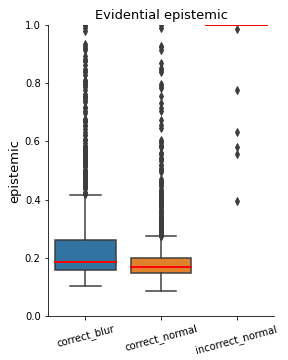
\includegraphics[width=0.35\linewidth]{images/blur_epistemic_normal.png}
	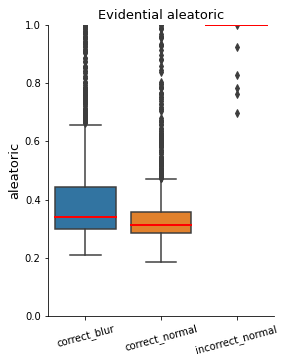
\includegraphics[width=0.35\linewidth]{images/blur_aleatoric_normal.png}
	\caption[Disentanglement of uncertainty for blur constraint]{Comparison of epistemic and aleatoric uncertainty for the blur constraint.}
	\label{fig:overview}
\end{figure}

\section{Datasets}

\begin{figure}
    \centering
    \includegraphics[width=8cm,height=8cm]{images/Normal_dataset.png}
    \caption{Dataset for normal conditions}
    \label{fig:normal_dataset}
\end{figure}

\begin{figure}
    \centering
    \includegraphics[width=8cm,height=8cm]{images/Bright_dataset.png}
    \caption{Dataset for bright lighting constraint}
    \label{fig:bright_dataset}
\end{figure}

\begin{figure}
    \centering
    \includegraphics[width=8cm,height=8cm]{images/Dark_dataset.png}
    \caption{Dataset for dark lighting constraint}
    \label{fig:dark_dataset}
\end{figure}

\begin{figure}
    \centering
    \includegraphics[width=8cm,height=8cm]{images/Far_dataset.png}
    \caption{Dataset for far distance constraint}
    \label{fig:far_dataset}
\end{figure}

\begin{figure}
    \centering
    \includegraphics[width=8cm,height=8cm]{images/Near_dataset.png}
    \caption{Dataset for near distance constraint}
    \label{fig:near_dataset}
\end{figure}

\begin{figure}
    \centering
    \includegraphics[width=8cm,height=8cm]{images/Textures_dataset.png}
    \caption{Dataset for textures constraint}
    \label{fig:textures_dataset}
\end{figure}

\begin{figure}
    \centering
    \includegraphics[width=8cm,height=8cm]{images/Deformation_dataset.png}
    \caption{Dataset for deformation constraint}
    \label{fig:deformation_dataset}
\end{figure}

\begin{figure}
    \centering
    \includegraphics[width=8cm,height=8cm]{images/Blur_dataset.png}
    \caption{Dataset for blur constraint}
    \label{fig:blur_dataset}
\end{figure}

\section{Tables}
% Please add the following required packages to your document preamble:
% \usepackage{multirow}
\begin{table}[]
\caption{Accuracy results of the four uncertainty estimation methods for all the test constraints}
\label{tab:accuracy_table}
\begin{tabular}{|c|c|c|c|c|c|}
\hline
Metric                    & Constraint  & Cross entropy & Evidentail & Dropout & Ensembles \\ \hline
\multirowP{}{Accuracy} & Normal      & 0.979         & 0.966      & 0.973   & 0.975     \\ \cline{2-6} 
                          & Far         & 0.324         & 0.375      & 0.311   & 0.285     \\ \cline{2-6} 
                          & Near        & 0.214         & 0.273      & 0.211   & 0.224     \\ \cline{2-6} 
                          & Bright      & 0.973         & 0.943      & 0.919   & 0.962     \\ \cline{2-6} 
                          & Dark        & 0.214         & 0.273      & 0.211   & 0.224     \\ \cline{2-6} 
                          & Textures    & 0.721         & 0.731      & 0.683   & 0.743     \\ \cline{2-6} 
                          & Deformation & 0.749         & 0.787      & 0.745   & 0.768     \\ \cline{2-6} 
                          & Blur        & 0.752         & 0.686      & 0.753   & 0.740     \\ \hline
\end{tabular}
\end{table}

\bibliography{demo.bib}

